\section{Tipos, Estruturas e Representações de Grafos}

\begin{frame}[plain]
  \centering
  \Huge \insertsection
\end{frame}

\begin{frame}{Grafo não Direcionado e sem Peso}
  \centering
  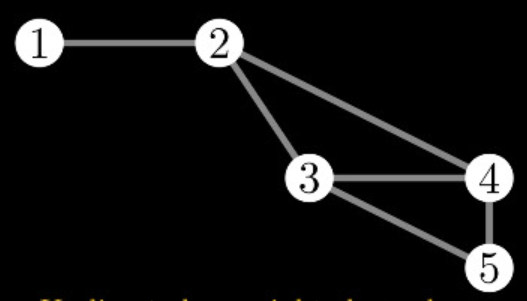
\includegraphics[width=1\textwidth]{./images/uduwgraph.png}
\end{frame}

\begin{frame}{Grafo não Direcionado e com Peso}
  \centering
  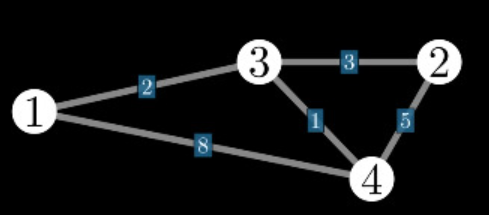
\includegraphics[width=1\textwidth]{./images/unwgraph.png}
\end{frame}

\begin{frame}{Grafo Direcionado e sem Peso}
  \centering
  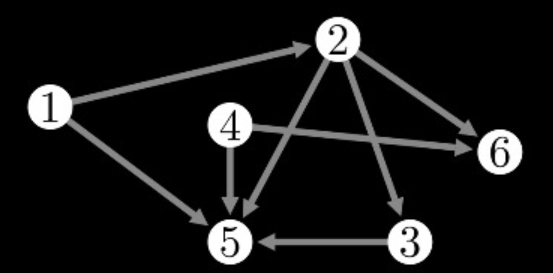
\includegraphics[width=1\textwidth]{./images/dungraph.png}
\end{frame}

\begin{frame}{Grafo Direcionado e com Peso}
  \centering
  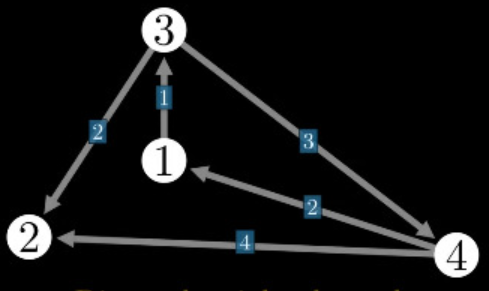
\includegraphics[width=1\textwidth]{./images/dwgraph.png}
\end{frame}

\begin{frame}{Representações de Grafos}
  \begin{itemize}
    \item \textbf{Lista de Adjacência:} Cada vértice possui uma lista de seus vizinhos.
    \item \textbf{Matriz de Adjacência:} Matriz onde cada célula indica a presença de uma aresta entre dois vértices.
    \item \textbf{Matrix de Incidência:} Matriz onde linhas representam arestas e colunas vértices, indicando a incidência de arestas em vértices.
  \end{itemize}
\end{frame}

\begin{frame}{Outros Tipos de Grafos}
  \begin{itemize}
    \item \textbf{Grafo Completo:} Todos os pares de vértices estão conectados por uma aresta.
    \item \textbf{Grafo de Euler:} Contém um ciclo que visita cada aresta exatamente uma vez.
    \item \textbf{Grafo de Hamilton:} Contém um ciclo que visita cada vértice exatamente uma vez.
    \item \textbf{Grafo Bipartido e K-partido:} Vértices podem ser divididos em dois ou mais conjuntos, onde arestas só conectam vértices de conjuntos diferentes.
    \item \textbf{Grafo Desconexo:} Não é possível alcançar todos os vértices a partir de um único vértice.
  \end{itemize}
\end{frame}